\documentclass[12pt]{article}
\usepackage{mathtools}
\usepackage{amsmath}
\usepackage{algorithmic}
\usepackage{algorithm}
\usepackage{float}
\setcounter{section}{0}
\begin{document}
    Nous allons comparer les quatres métaheuristiques implémentées afin de voir l’apport de chaque méthode en terme de qualité de solution et de temps d'exécution.

    Tout d’abord nous allons vous rappeler les métriques de cette comparaison, ainsi que la formule de chacune :
    \begin{itemize}
        \item \textbf{Temps d'exécution moyen} : la moyenne des temps d'exécution pour toutes les instances ayant la même valeur du N, le nombre d’objets.
        \item \textbf{La moyennes des écarts de la solution optimale} : pour chaque instance on calcule 
        \((n\_bins - opt)*100/opt\) avec \(n\_bins\) nombre de boîtes obtenu par la métaheuristique et \(opt\) nombre de boîtes dans la solution optimale, puis on calcule la moyenne de ces écarts pour les instances ayant le même nombre d’objets, hormis la classe HARD qui a été séparée des autres, vu le degré de difficulté de ces instances. 
    \end{itemize}

    Il est à noter que les résultats des algorithmes AG, et RS sont le résultats de dix exécutions par instance, afin d’échapper à l’aspect aléatoires des fonctions intérieures à ces deux méthodes, où le temps d'exécution moyen et la meilleure solution parmis les dix obtenues ont été pris
    Dans ce qui suit on va comparer:
    \begin{itemize}
        \item Whale Optimization Algorithm (WOA).
        \item Improved Whale Optimization Algorithm (ILWOA).
        \item L’Algorithm Génétique (AG).
        \item Recuit Simulé (RS).
    \end{itemize} 
    \subsection{Comparaison par rapport au temps d'exécution}
        \begin{figure}[H]
            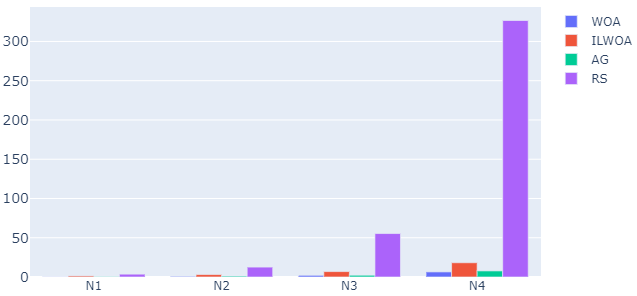
\includegraphics[width=\linewidth]{../figures/mh_texec.png}
            \caption{la moyenne des temps d'exécution (en s) des métaheuristiques en fonction de la taille d'instance}
        \end{figure}
        \subsubsection{Analyse et interprétation}
            \begin{itemize}
                \item On peut clairement voir à partir du  graphe ci-dessus que le recuit simulé (RS) est l’algorithme le plus lent des quatre algorithmes, et dont le temps d'exécution augmente avec l’augmentation de la taille des instances. 
                \item l’algorithm génétique (AG)  est la méthode la plus rapide suivi du WOA en deuxième position, et ILWOA juste derrière.
                \item Contrairement à ce que le graphe montre, l’algorithme ILWOA converge beaucoup plus rapidement que WOA .En effet, le temps d'exécution ne reflète pas exactement la vitesse de convergence d’un algorithme dans notre cas dû au choix de la condition d'arrêt qui est pour rappel le nombre d'itérations (section ILWOA).
                \item Le temps d'exécution des métaheuristiques est plus grand que le temps d'exécution des heuristiques, et ceci est triviale, à cause de la nature gloutonne des heuristiques, contrairement aux métaheuristiques qui sont des méthodes plus sophistiqués,utilisant plusieurs mécanismes d’intensification et diversification pour éviter les optimums locaux.
            \end{itemize}
    \subsection{Comparaison par rapport à la qualité de la solution}
        \begin{figure}[H]
            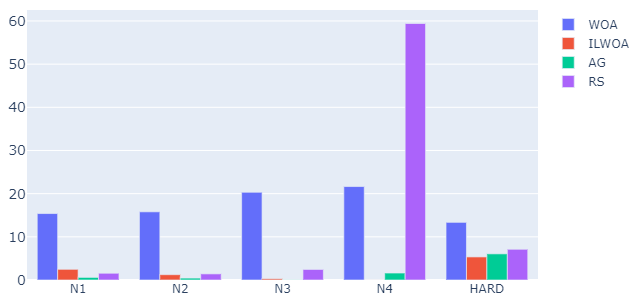
\includegraphics[width=\linewidth]{../figures/mh_ecart.png}
            \caption{la moyenne des écarts (en \%) des métaheuristiques de la solution optimale en fonction de la taille d'instance}
        \end{figure}
        \subsubsection{Analyse et interprétation}
            \begin{itemize}
                \item On remarque que WOA dans tous les cas donne le plus grand écart par rapport à la solution optimale sauf dans le cas N4=500 où c’est RS qui trouve les solutions les plus écartées des solutions optimales (un écart de 60%). 
                \item Pour la majorité des tailles des instances, AG donne les meilleurs résultats sauf dans le cas des instances Hard et N4 où ILWOA offre une légère amélioration. On peut donc conclure qu'en général AG donne de meilleurs solutions pour toutes les instances du benchmark. et ILWOA est celui qui arrive à améliorer les solutions des instances HARD. 
                \item Les solutions obtenues sont généralement proches de celles retournées par les heuristiques, avec quelques instances où les métaheuristiques sont meilleures que les heuristique et vise versa.
            \end{itemize}
            Enfin, d’après ces deux graphes synthétiques, on conclut  que AG donne de meilleurs résultats en faisant un compromis entre le temps d'exécution et la qualité de la solution, le ILWOA pas très loin derrière.
\end{document}